\documentclass[border=1pt]{standalone}
\usepackage[scaled=0.92]{helvet}
\renewcommand{\familydefault}{\sfdefault}
\usepackage{amsmath}
\usepackage{tikz}
\usetikzlibrary{arrows.meta,fit,calc,backgrounds}
\definecolor{nn}{HTML}{F6C6A8}\definecolor{nnline}{HTML}{D9825B}
\definecolor{nonnn}{HTML}{A9D2F1}\definecolor{nonnnline}{HTML}{4F95CF}
\definecolor{panel}{HTML}{EDEDED}\definecolor{txt}{HTML}{333333}
\begin{document}
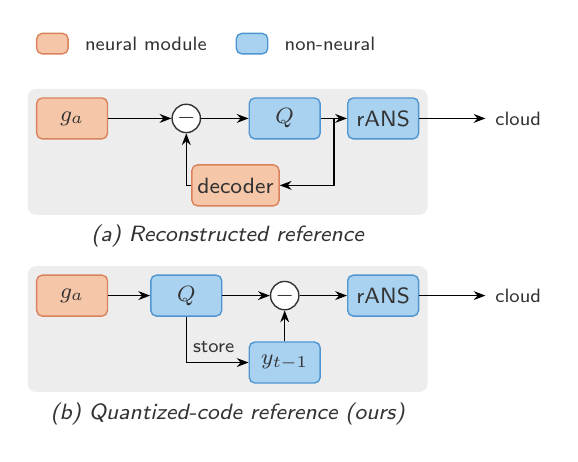
\begin{tikzpicture}[
  font=\footnotesize, text=txt,
  >={Stealth[length=1.5mm]}, line width=0.5pt,
  box/.style={rounded corners=2pt, minimum height=5.2mm, minimum width=9mm, inner sep=2pt, align=center},
  nnb/.style={box, fill=nn, draw=nnline},
  pb/.style={box, fill=nonnn, draw=nonnnline},
  op/.style={circle, draw=txt, fill=white, inner sep=0pt, minimum size=3.6mm},
  pan/.style={fill=panel, rounded corners=3pt, inner sep=3pt},
  subcap/.style={font=\footnotesize\itshape, anchor=north},
]
% shared column positions (cm)
\def\cA{0}\def\cB{1.45}\def\cC{2.7}\def\cD{3.95}\def\cE{5.25}
\def\rowgap{-0.85}

% legend
\node[nnb, minimum width=4mm, minimum height=2.6mm] (l1) at (\cA-0.25,0.95) {};
\node[anchor=west, font=\scriptsize] (l1t) at ($(l1.east)+(0.08,0)$) {neural module};
\node[pb, minimum width=4mm, minimum height=2.6mm] (l2) at ($(l1t.east)+(0.45,0)$) {};
\node[anchor=west, font=\scriptsize] at ($(l2.east)+(0.08,0)$) {non-neural};

% ---------- (a) reconstructed reference ----------
\node[nnb] (a1) at (\cA,0) {$g_a$};
\node[op]  (a2) at (\cB,0) {$-$};
\node[pb]  (a3) at (\cC,0) {$Q$};
\node[pb]  (a4) at (\cD,0) {rANS};
\node[nnb] (a5) at ($(\cB,\rowgap)!0.5!(\cC,\rowgap)$) {decoder};
\coordinate (a6) at (\cE,0);
\draw[->] (a1)--(a2); \draw[->] (a2)--(a3); \draw[->] (a3)--(a4);
\draw[->] (a4)--(a6) node[right, font=\scriptsize]{cloud};
\draw[->] ($(a3.east)!0.5!(a4.west)$) |- (a5.east);
\draw[->] (a5.west) -| (a2.south);
\begin{scope}[on background layer]
\coordinate (aL) at (\cA-0.45,0); \coordinate (aR) at (\cD+0.45,0);
\node[pan, fit=(a1)(a4)(a5)(aL)(aR)] (pa) {};
\end{scope}
\node[subcap] at (pa.south) {(a) Reconstructed reference};

% ---------- (b) quantized-code reference ----------
\begin{scope}[yshift=-2.25cm]
\node[nnb] (b1) at (\cA,0) {$g_a$};
\node[pb]  (b2) at (\cB,0) {$Q$};
\node[op]  (b3) at (\cC,0) {$-$};
\node[pb]  (b4) at (\cD,0) {rANS};
\node[pb]  (b5) at (\cC,\rowgap) {$y_{t-1}$};
\coordinate (b6) at (\cE,0);
\draw[->] (b1)--(b2); \draw[->] (b2)--(b3); \draw[->] (b3)--(b4);
\draw[->] (b4)--(b6) node[right, font=\scriptsize]{cloud};
\draw[->] (b2.south) |- node[pos=0.72, above, font=\scriptsize]{store} (b5.west);
\draw[->] (b5)--(b3);
\begin{scope}[on background layer]
\coordinate (bL) at (\cA-0.45,0); \coordinate (bR) at (\cD+0.45,0);
\node[pan, fit=(b1)(b4)(b5)(bL)(bR)] (pnb) {};
\end{scope}
\node[subcap] at (pnb.south) {(b) Quantized-code reference (ours)};
\end{scope}
\end{tikzpicture}
\end{document}
